\documentclass[12pt,a4paper]{article}
%police
\usepackage[utf8]{inputenc}
\usepackage[T1]{fontenc}
\usepackage[french]{babel}

\usepackage[tc]{titlepic}

\usepackage{adjustbox}
\usepackage{graphicx}
\usepackage{layout}
\usepackage{fancyhdr}
\usepackage{eurosym}
\usepackage{multirow}
\usepackage{float}
\usepackage[normalem]{ulem}

\usepackage{hyperref}

\usepackage{geometry}
\geometry{margin=1.2in}

\pagestyle{fancy}
\fancyhead{}
\renewcommand{\headrulewidth}{0pt}
\lfoot{PLT - BALACHANDRAN Chirojean - FAUJEAU François}
\cfoot{}
\rfoot{\thepage}

\begin{document}

\begin{titlepage}

\newcommand{\HRule}{\rule{\linewidth}{0.5mm}} % Defines a new command for the horizontal lines, change thickness here

\begin{minipage}{0.4\textwidth}
\begin{flushleft} \large

\includegraphics[width=0.5\textwidth]{Logo_ENSEA.jpg} 
\end{flushleft}
\end{minipage}
~
\begin{minipage}{0.57\textwidth}
\begin{flushright} \large
FAUJEAU François \textsc{} \\
BALACHANDRAN Chirojean\textsc{} \\
3A IS\textsc{} \\
\end{flushright}
\end{minipage}\\[1cm]

\centering

\HRule \\[0.5cm]
{ \huge \bfseries PROJET CIVILIZATION}\\[0.3cm]% Title of your document
Rapport du projet logiciel transversal \textsc{} \\[0.5cm]
\HRule \\[3cm]


\includegraphics[width=1\textwidth]{ressources/map.png}\\[3.5cm]


\begin{flushleft}
Année scolaire: 2018-2019
\end{flushleft}
\end{titlepage}


\newpage

\tableofcontents
\thispagestyle{empty}
\setcounter{page}{0}

\newpage

\section{Présentation générale}

\subsection{Archétype}

Le but de notre projet logiciel transversal est de créer une version très simplifiée du jeu civilization. Ce jeu est un jeu de stratégie tour par tour où l'objectif d'un joueur est de développer un empire en choississant une civilisation au choix parmi plusieurs. 

\begin{figure}[!ht]
    \centering
    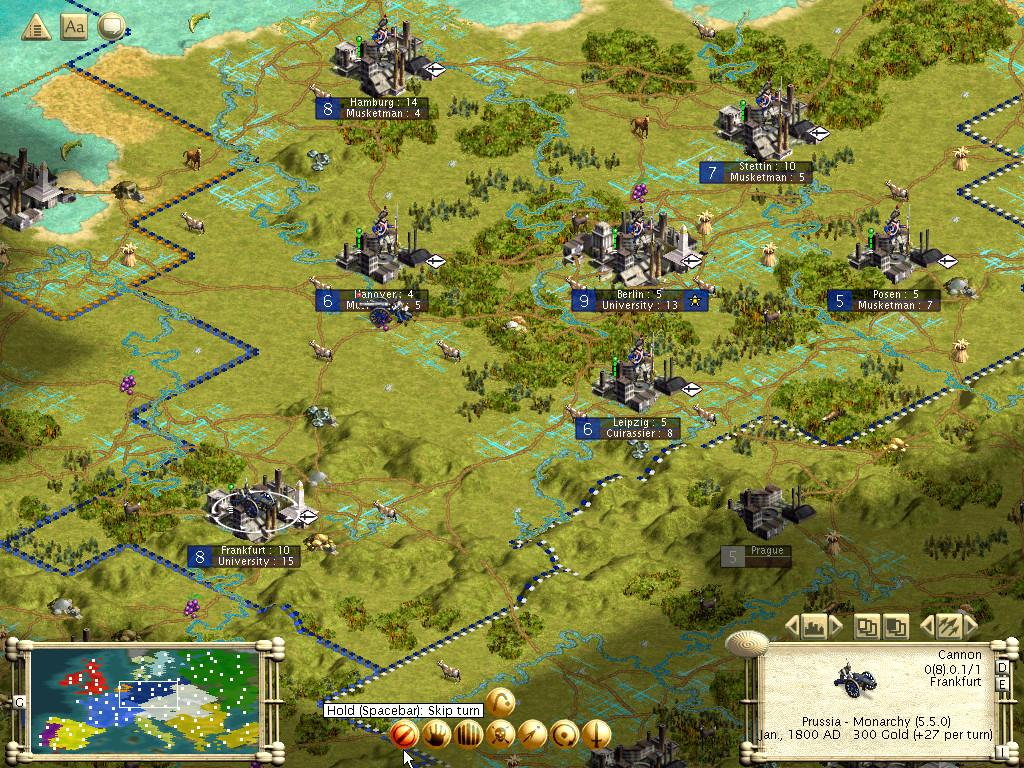
\includegraphics[width=0.7\textwidth]{civ3.png}
     \caption{Image d'un gameplay de civilization 3}
\end{figure}

\subsection{Règles du jeu}

Le but pour chaque joueur est de développer un empire avec la civilisation romaine. Pour cela, le joueur doit améliorer et gérer ses ressources (mines d'or, terres agricoles) ainsi que ses bâtiments (caserne et palais). \\
Nous avons choisi que chaque joueur pourrait seulement utiliser la civilisation romaine. Chaque empire permet de créer différents bâtiments : 
\begin{enumerate}
    \item Le palais : bâtiment principal de l'empire. Son niveau correspond au niveau de l'empire. Plus sont niveau est élevé et plus il est possible d'améliorer les autres bâtiments et unités.
    \item La caserne : permet de former des soldats. Quand le niveau de la caserne augmente, le niveau des troupes formées et le nombre des troupes qui peuvent être formées augmentent. Il y aura quatre types d'unités de combat : un cavalier, un épéiste, un archer et une catapulte. A la création d'une unité, le joueur choisira si elle est créée pour défendre l'empire ou si elle peut se déplacer sur la carte de jeu.
    \item Ressources : le joueur possèdera trois types de ressources à savoir les mines d'or, la réserve de bois et les terres agricoles. Quand le niveau d'une ressource augmente, la capacitée de stockage de cette ressource et la quantité produite sont augmentées.
\end{enumerate}
Pour améliorer les bâtiments, il faudra que le joueur dépense une certaine quantité de bois et d'or et pour la formation de soldats une certaine quantité de récoltes agricoles et d'or.\\
Pour développer son empire plus rapidement il est possible d'en combatre un autre (détenu soit par l'IA, soit par un joueur) ou de s'en défendre. En effet, en cas de victoire l'empire victorieux reçoit une partie des ressources de l'empire adverse et un bonus de victoire. L'empire qui a perdu recupère, lui, un faible bonus de défaite. \\Le système de combat est le suivant. 
Chacun leur tour, les joueurs pourront décider de : 
\begin{itemize}
    \item se déplacer pour se rapprocher du combat.
    \item choisir qu'un soldat en attaque un autre s'il est dans sa zone d'action.
\end{itemize}
Un combat se termine lorsque tous les soldats d'un joueur sont éliminés. 
\\Dans notre jeu, un tour correspond à une action: une amélioration de bâtiment, la formation d'une unité, son déplacement.\\

\subsection{Ressources}

Voici les différentes ressources (images, textures, sprites) utilisées pour le développement du jeu. Pour créer les cartes de jeu nous les génèrerons de manière aléatoire en mode isométrique. Ces cartes sont des cartes de jeu 25 x 25.

\begin{figure}[!ht]
    \centering
    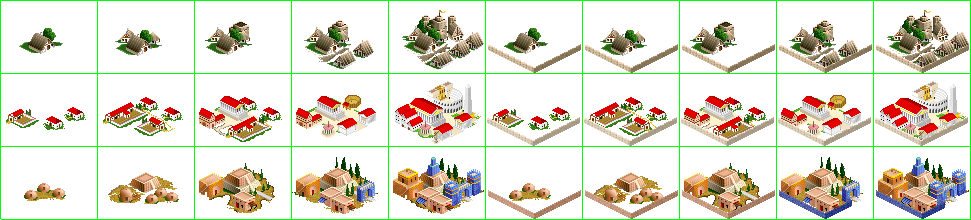
\includegraphics[width=0.7\textwidth]{ressources/cities2.png}
     \caption{Bâtiments de la civilisation romaine en fonction des niveaux}
\end{figure}

\begin{figure}[!ht]
    \centering
    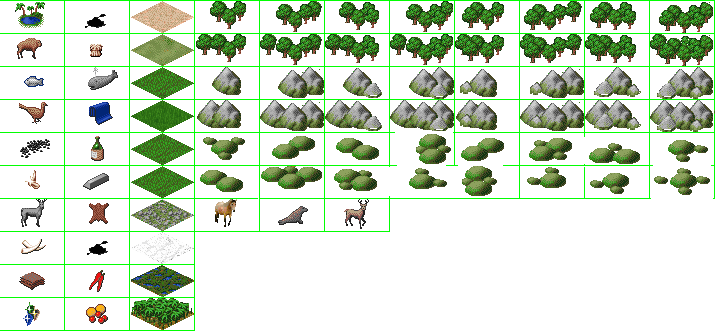
\includegraphics[width=0.7\textwidth]{ressources/Terrain.png}
     \caption{textures pour la création de la map}
\end{figure}
\newpage
\begin{figure}[!ht]
    \centering
    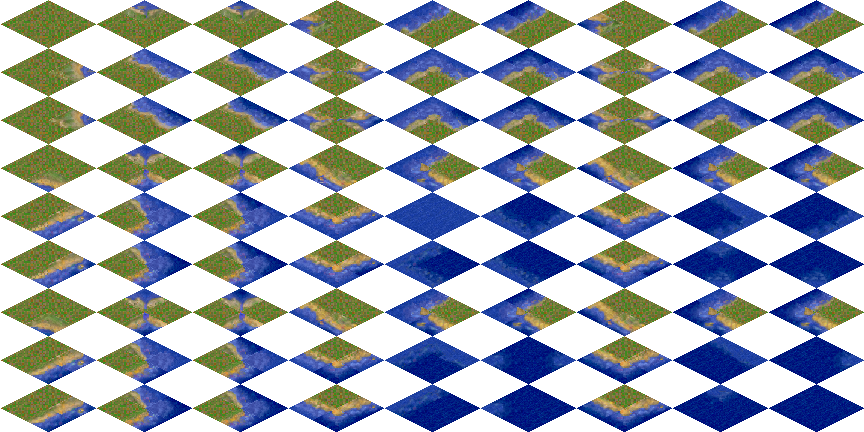
\includegraphics[width=0.7\textwidth]{ressources/ocean.png}
     \caption{textures pour la mer sur la map}
\end{figure}

\begin{figure}[!ht]
    \centering
    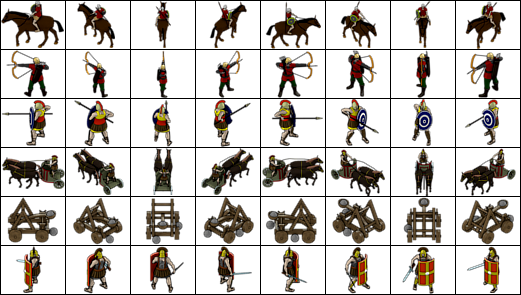
\includegraphics[width=0.7\textwidth]{ressources/Units.png}
     \caption{images des unités de combats}
\end{figure}

\newpage

\section{Description et conception des états}

\subsection{Description des états}

Un état de jeu est constitué d'une carte sur lequel se situent différents empires avec leurs différents bâtiments (éléments fixes), les éléments de décor (éléments fixes) et des unités de combats (éléments mobiles).

\subsubsection{Description de la carte}

La carte est représentée avec une grille composée de cases contenant des éléments sur chacunes d'elles avec une certaine position. Elle est composée d'empires, qui sont eux-mêmes constitués de bâtiments, et d'éléments comme les bâtiments, les unités de combats et les éléments de décor. Certains éléments sont franchissables par les unités et d'autres non. La taille de la carte est fixée.

\subsubsection{Description des états éléments fixes}

Les éléments fixes sont les décors et les bâtiments et les empires qui sont abstraits. Tous les éléments fixes possèdent une position (x,y) entre 0 et 24.\\

\uline{Décors}\\

Les décors sont de différents types: eau, herbe, dunes, montagnes, arbre, animaux... Ils ont chaucun un identifiant. Les décors possèdent un attribut passable qui permet de savoir si l'élément est franchissable ou non par les unités de soldats.\\

\uline{Empire}\\

Un empire a plusieurs attributs:
\begin{itemize}
\item un identifiant pour le différencier des autres empires (chiffre)
\item un nom
\item un niveau compris entre 1 et 4
\item des points de vie qui sont égaux à ceux du palais
\item des ressources (or, bois, nourriture) pour se développer et former des troupes
\item une liste de position permettant d'indiquer où se positionne l'empire sur la carte
\end{itemize}

Enfin, il est composée d'une caserne, d'un bâtiment ressource et enfin d'un palais. \\

\uline{Bâtiments}\\

Les bâtiments ont tous ces attributs :
\begin{itemize}
\item un identifiant pour le différencier des autres (chiffre)
\item un niveau qui va de 1 à 4
\item un coût en bois et en or pour les construire
\item un identifiant pour leur texture graphique
\end{itemize}

Il y a trois types de bâtiments: la caserne, les ressources et le palais.

La caserne a une capacité maximale de formation de troupes et possède comme attribut le nombre de troupes formées. Elle permet de former les différentes troupes.

Les ressources ont un niveau de production identique pour l'or, le bois ainsi que la nourriture. Ils vont permettre d'augmenter la richesse d'un joueur à chaque tour.

Le palais quant à lui possède des points de vie. C'est lui qui sera attaqué par un joueur et sa destruction mènera à la fin d'une partie.\\

Une carte de jeux typique sera composée de 25 x 25 cases disposées de manière isométrique. Ces cartes seront générées de manière aléatiores. 

\subsubsection{Description des états éléments mobiles}\\

Tous les éléments mobiles possèdent une position (x,y). 
Ils possèdent tous:
\begin{itemize}
\item un identifiant pour les différencier
\item un niveau de vie
\item un niveau de dommages en attaque
\item une portée pour attaquer
\itemun nombre de déplacements de cases limité
\item un coût en or et en nourriture pour la former
\item un identifiant de texture graphique.
\end{itemize}
Les unités de soldats dans le jeu sont les unités de combats: décurion, cavalier, catapulte et archer.\\

\subsection{Conception des états}
Dans cette partie nous allons décrire le diagramme UML d'état du jeu. (Voir figure 6)\\

Class "Element" : Cette classe est la classe mère de tous nos éléments, mobiles ou statiques. Nous avons choisi pour cette classe qu'elle contienne une position, la position de notre élément sur la map, et une méthode isPassable(), qui nous permet de savoir si l'élément peut être traversé par un autre.\\

Class "Units" : Cette classe est la classe mère de toutes nos unités mobiles sur la carte. Elle hérite d'"Element". Elle contient tous les paramètres nécessaires à la création d'une unité (vie, attaque, niveau, ...). \\

Class "Arrow" : Cette classe est la classe fille de Units. Elle hérite d'"Element". Elle permet de construire des unitées de type archer avec leurs attributs initialisés en fontion de leur niveau. Ce sera la façon la plus utilisée de créer un archer. Il existe de même des classes pour Decurion, Cavalier et Catapult.\\

Class "Buildings" : Cette classe est la classe mère de toutes nos unités statiques sur la carte. Elle hérite d'"Element". Elle contient tous les paramètres nécessaires à la création d'un bâtiment (niveau, coût, ...).\\

Class "Barrack" : Une caserne est un bâtiment et hérite donc de "Buildings", elle ajoute en plus quelques fonctionnalitées telles que la création d'unités. De même pour les bâtiments de type ressource et palais.\\

Concernant les coûts, nous avons créé deux classes qui permettent de créer le coût des unités et des bâtiments, et de pouvoir les modifier.\\

Nous avons aussi choisi d'attribuer à chaque élément un id qui permet de savoir instantanément lequel il est.\\

Class "Decor" : Cette classe hérite d'élément, elle permet de créer les différents décors qui seront présents sur la carte de jeu.\\ 

Class "Empire" : Dans notre jeu nous avons besoin à tout instant d'avoir une classe qui stocke les éléments importants d'un empire. Par exemple un empire à un nom, une vie, de l'or, du bois, de la nourriture, ... . Ainsi, cette classe va agir comme un conteneur de tous les élements clés de notre empire.\\

Class "Map" : cette classe contient les éléments sur la carte de jeu. Elle permet d'ajouter des éléments, de les récupérer ou d'en supprimer.\\

Class "Observable" : cette classe permet de réagir au des actions gérées par le moteur de jeu. Par exemple, lorsqu'un joueur souhaite améliorer un bâtiment ou créer une unité sur la carte de jeu, il faut que les cartes contenues dans notre classe Map soient modifées en conséquence.\\ Elle contient une méthode appelée "notifyObserveur" qui va notifier ses observeurs. Cet observable est composé de deux observeurs : UnitsObserver et BuildingsObserver.\\

Class "UnitsObserver" : Cette classe est un Observer sur les Units. Elle va permettre de réaliser tous les changements nécessaires sur le state des units demandés par le moteur.

Class "BuildingsObserver" : Cette classe est un Observer sur les Buildings. Elle va permettre de réaliser tous les changements nécessaires sur le state des buildings demandés par le moteur.

\begin{figure}[!ht]
\centering
    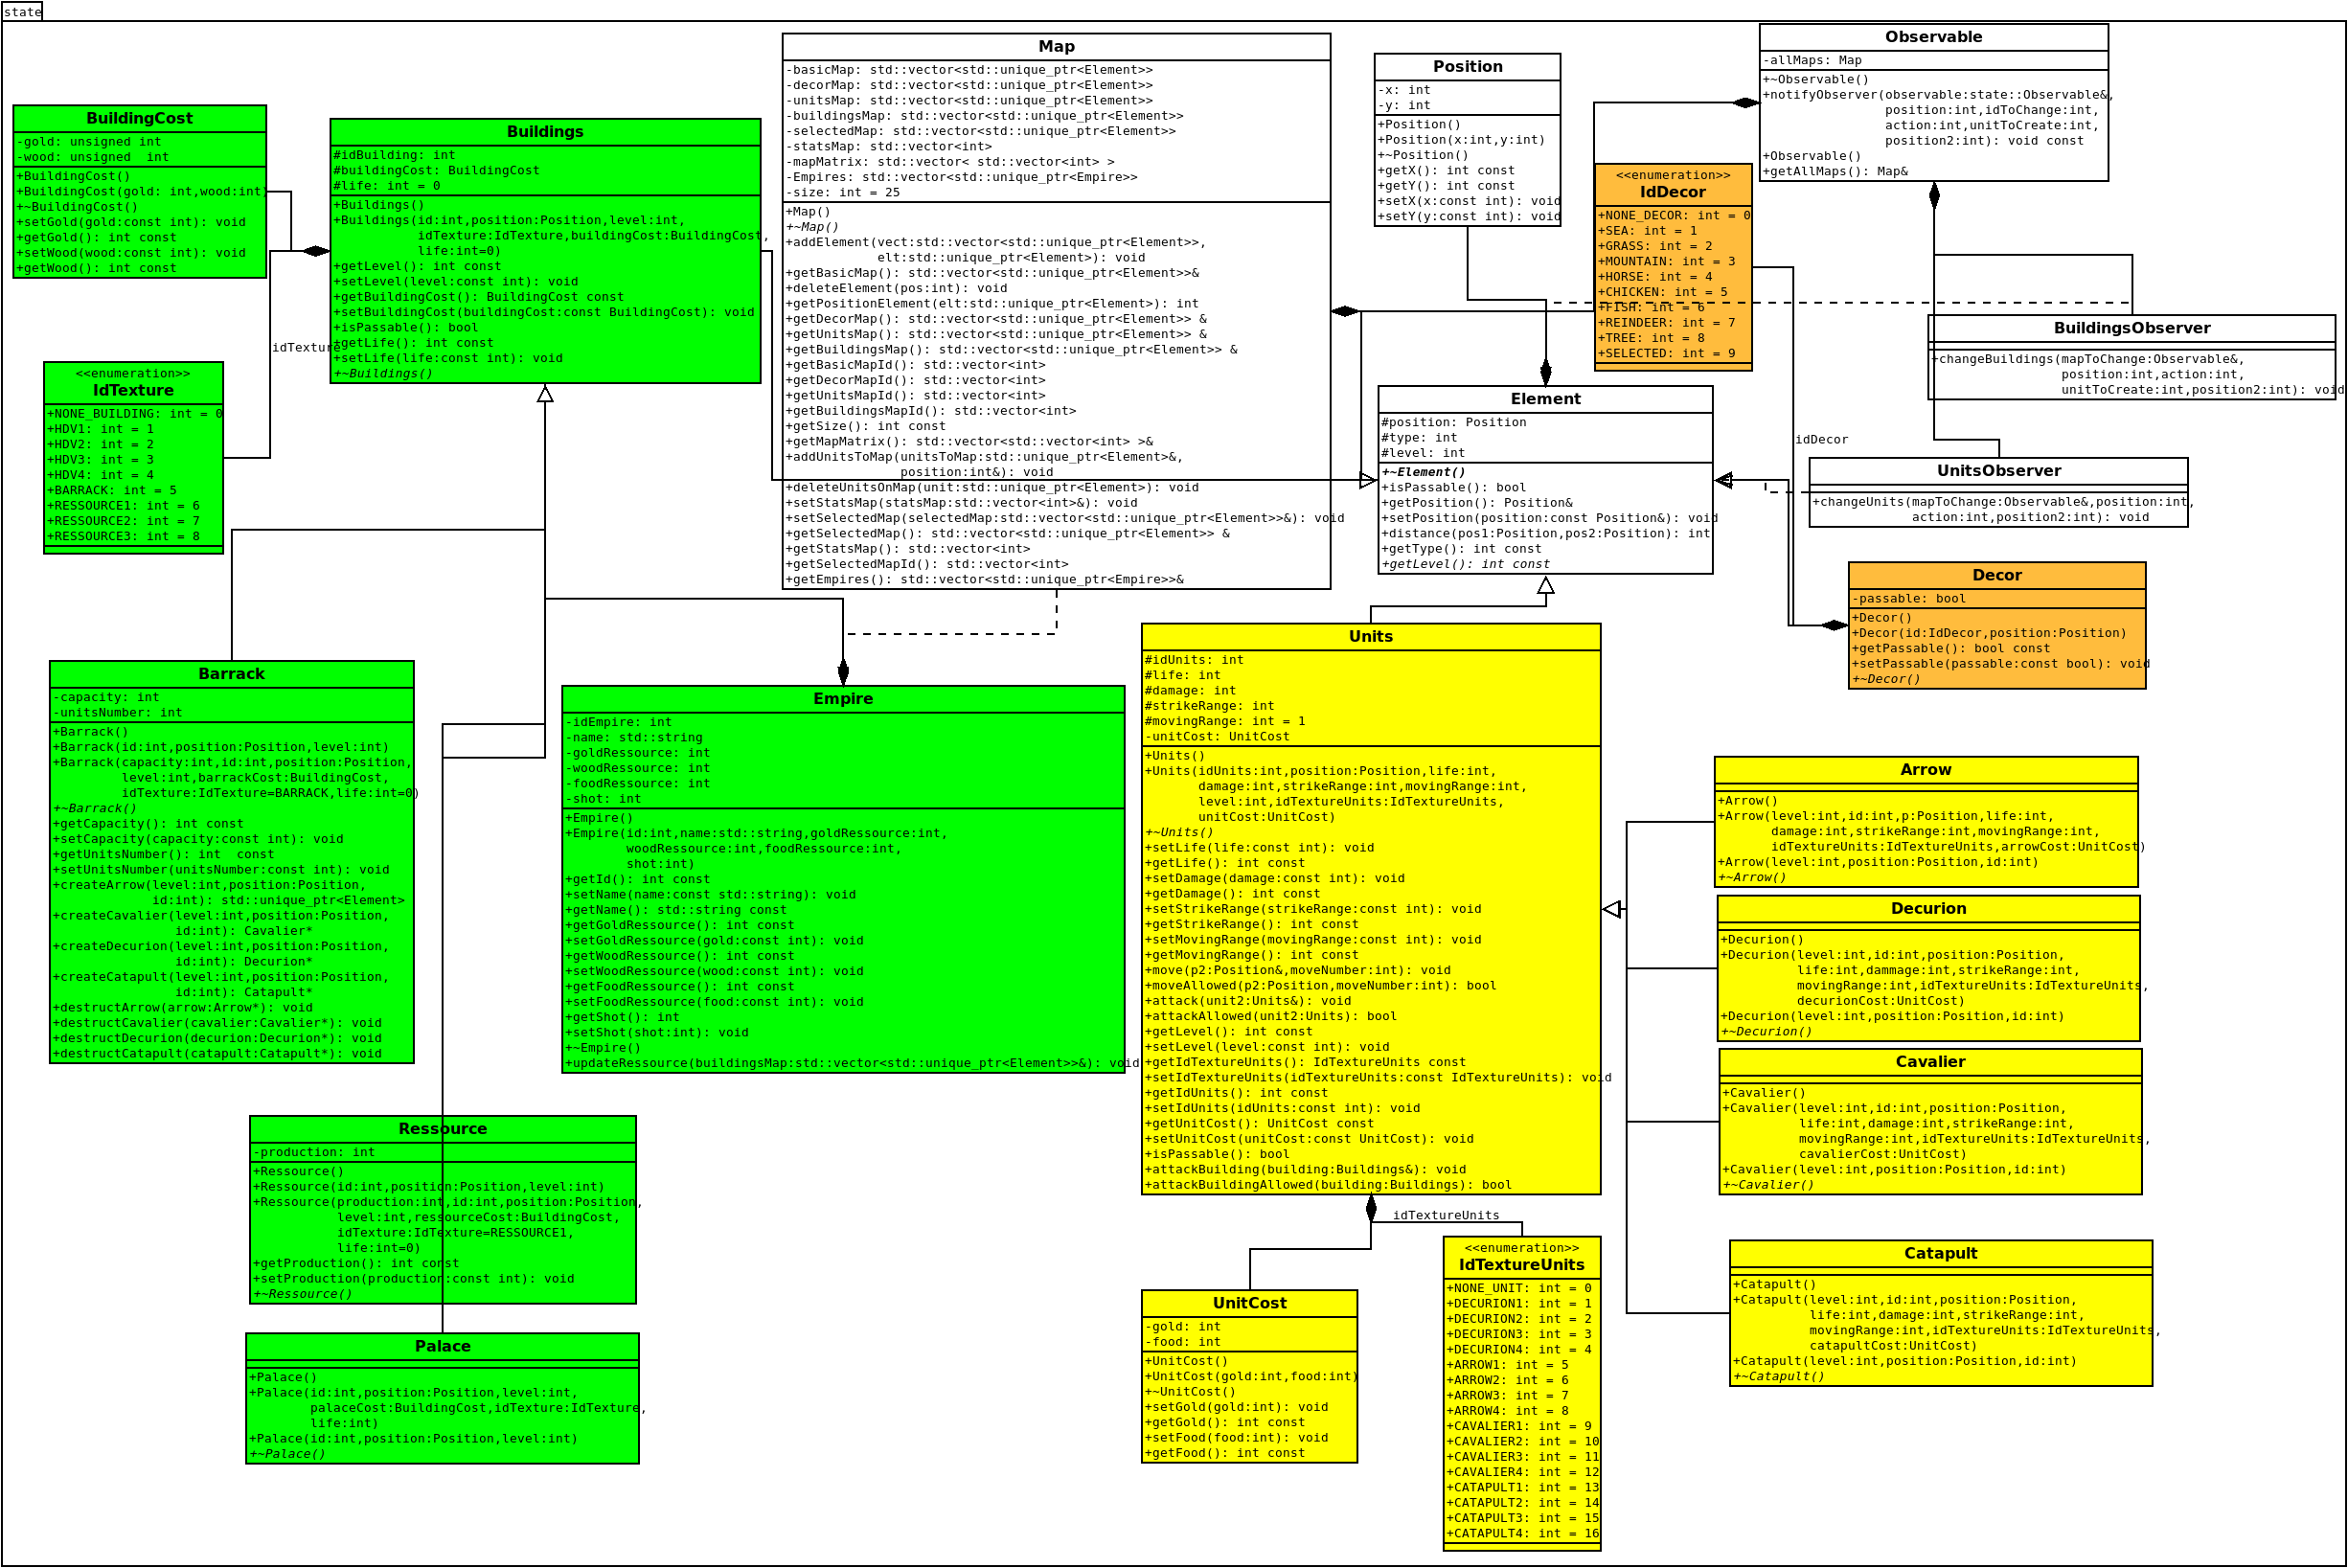
\includegraphics[width=1\textwidth]{ressources/state.png}
     \caption{Diagramme de classes d'état}
\end{figure}

\newpage
 '
\newpage
\section{Rendu: Stratégie et conception des états}
\subsection{Stratégie de rendu d'un état}

Pour le rendu des états, nous avons décidé de faire une carte en 2D avec des tuiles et en isométrie. Cette carte sera à chaque fois générée aléatoirement et donc à chaque lancement du programme elle sera différente. Nous utilisons la librairie SFML. Nous avons trois tilesets qui vont nous servir à créer les textures de la carte: 
\begin{itemize}
\item un pour les textures du terrain (eau, herbe, animaux ...)
\item un pour les bâtiments (caserne, ressource, palais)
\item un pour les unités (archer, cavalier, decurion, catapulte)
\end{itemize}\\

Sur le côté gauche, un petit menu permet de donner le niveau, la vie et les dommages s'il y en a des éléments.

Nous aurons une carte divisée en quatre plans: 
\begin{itemize}
\item un pour l'herbe et l'eau qui sont nos éléments visuels de base
\item un pour les éléments de décor comme les montagnes, les arbres ou encore les animaux
\item un pour les bâtiments
\item un pour les unités mobiles
\end{itemize}\\

Les trois premiers plans seront initialisés au départ du jeu grâce aux textures et à des tableaux constitués des numéros de texture d'éléments, selon une position, générés aléatoirement, selon certaines règles de création de map:
\begin{itemize}
\item Toute la carte est préalablement constitué d'herbe seulement
\item Ensuite, trois zones d'eau sont tirées au sort aléatoirement
\item Puis, trois zones d'arbres et de montagnes sont tirées  aléatoirement et quelques animaux sont placés
\item Enfin, trois positions pour les empires sont tirées au sort et les trois bâtiments sont placés côte à côte
\end{itemize}\\

Tous les plans seront ensuite superposés pour former la carte. Les troix premiers plans seront fixes et seul le plan des unités changera. Ce dernier sera en effet modifié à chaque tour lorsque l'utilisateur fera déplacer ses unités mobiles. La mise à jour de l'affichage et du changement d'états se fera à une fréquence de quelques hertz.

\newpage

\begin{figure}[!ht]
\centering
    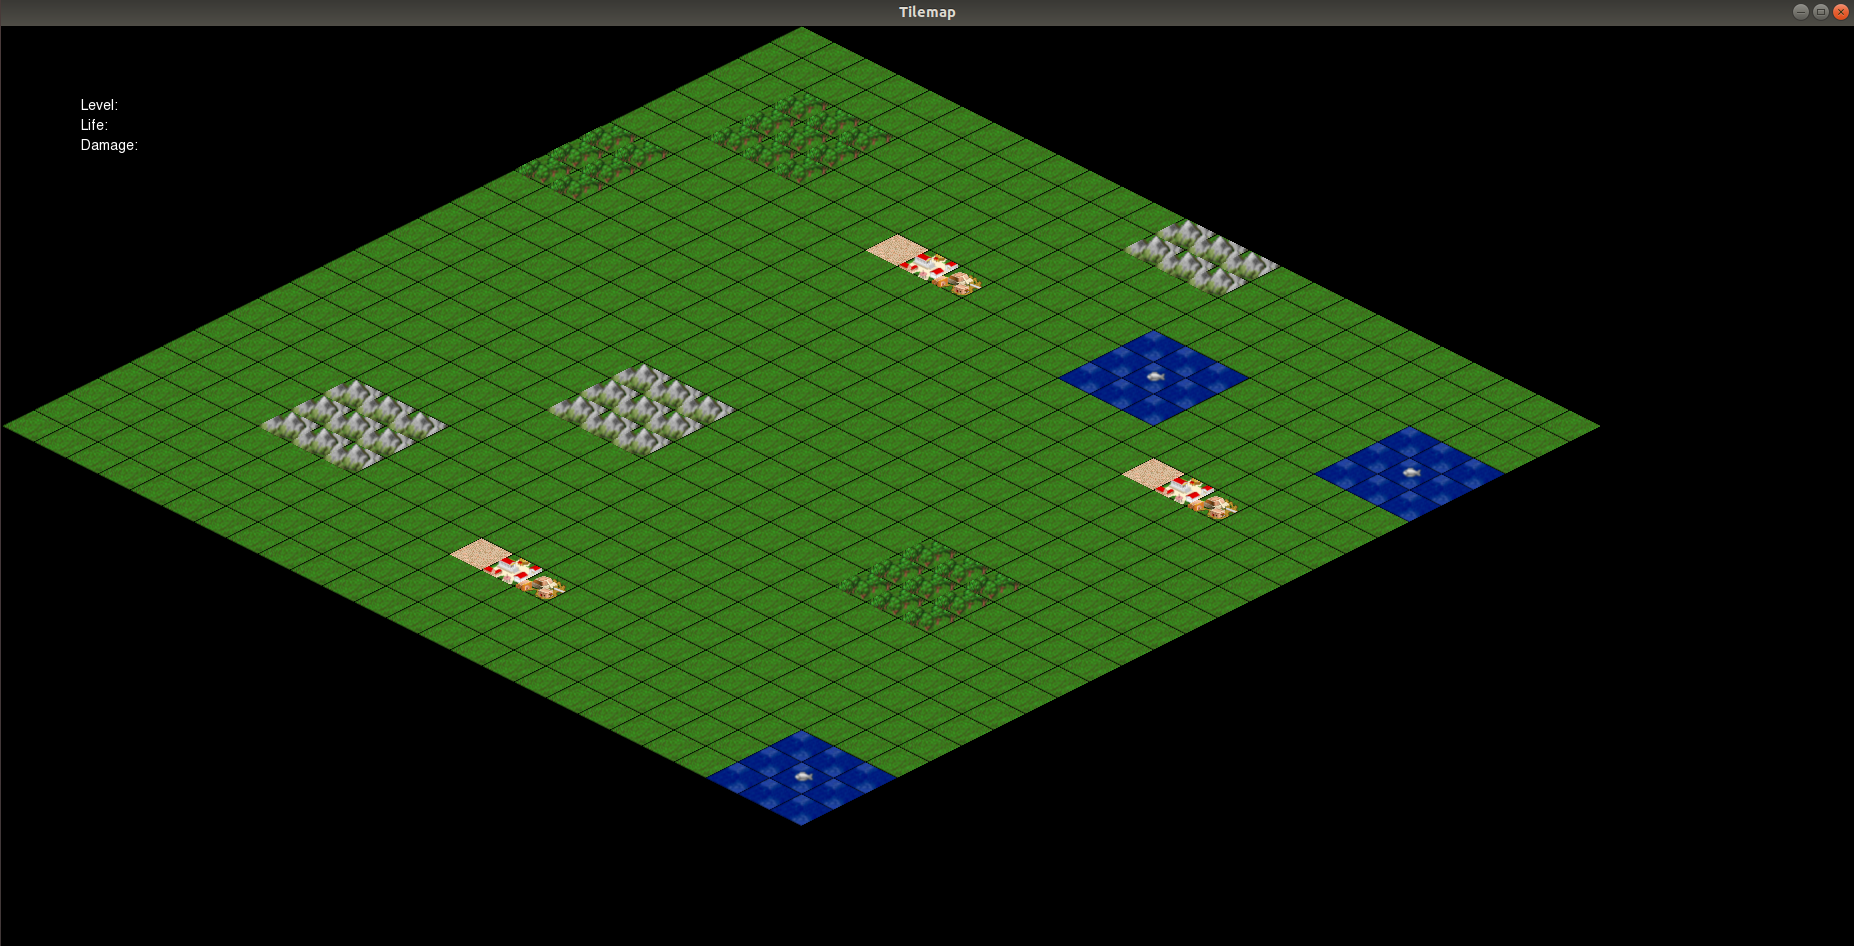
\includegraphics[width=1\textwidth]{ressources/MapAlea.png}
     \caption{Exemple d'un état généré aléatoirement}
\end{figure}

\subsection{Conception de rendu d'un état}
Dans cette partie nous allons décrire le diagramme UML de rendu d'un état du jeu.

Class "Tiles" : C'est un élément de base des tilesets. Ils ont une longueur et une largeur comme attributs ainsi qu'une position dans le tileset.

Class "TileSet" : Cette classe est la classe mère de tous les tilesets (tableaux de tuiles associés aux éléments). Elle est composée de tuiles. Nous avons choisi pour cette classe qu'elle contienne une méthode pour connaître la largeur d'une tuile et une autre qui permet de renvoyer la hauteur d'une tuile.\\

Class "BuildingTileSet" :  Elle hérite de "TileSet". Elle contient trois tableaux de tuiles comme attributs (un pour les casernes, un pour les palais et un pour les ressources) permettant de donner la texture associée à chaque élément. Elle possède une méthode permettant de renvoyer le chemin du fichier png contenant le tileset et une autre pour obtenir la tuile d'un bâtiment donné. \\

Class "DecorTileSet" :  Elle hérite de "TileSet". Elle contient un tableau de tuiles pour les décors comme attributs permettant de leur donner la texture associée. Elle possède une méthode permettant de renvoyer le chemin du fichier png contenant le tileset et une autre pour obtenir la tuile d'un décor donné. \\

Class "UnitsTileSet" :  Elle hérite de "TileSet". Elle contient quatre tableaux de tuiles comme attributs (un pour les archers, un pour les cavaliers, un pour les décurions et un pour les catapultes) permettant de donner la texture associée à chaque unité. Elle possède une méthode permettant de renvoyer le chemin du fichier png contenant le tileset et une autre pour obtenir la tuile d'une unité donnée. \\

Class "MapCreator" : Cette classe permet de créer une carte avec des textures d'un tileset. Elle constitue les plans d'une carte. Elle contient des textures et un tableau en attributs. Elle a des méthodes pour charger un fichier de texture, d'initialiser lee tableau, pour positionner un sprite sur une carte et lui donner sa texture et enfin d'afficher cette carte.\\

Class "MenuLayer" : Cette classe permet le menu permettant d'indiquer le niveau, la vie et les dommages.

Class "Layer" : Cette classe permet de créer des plans de carte. Elle est composée de MapCreator. Elle a comme attributs les tableaux de textures, selon leurs position, des éléments de base (herbe, eau), des décors et des bâtiments. Elle fait le lien entre la map du jeu contenue dans le diagramme d'état et le rendu.\\



\begin{figure}[!ht]
\centering
    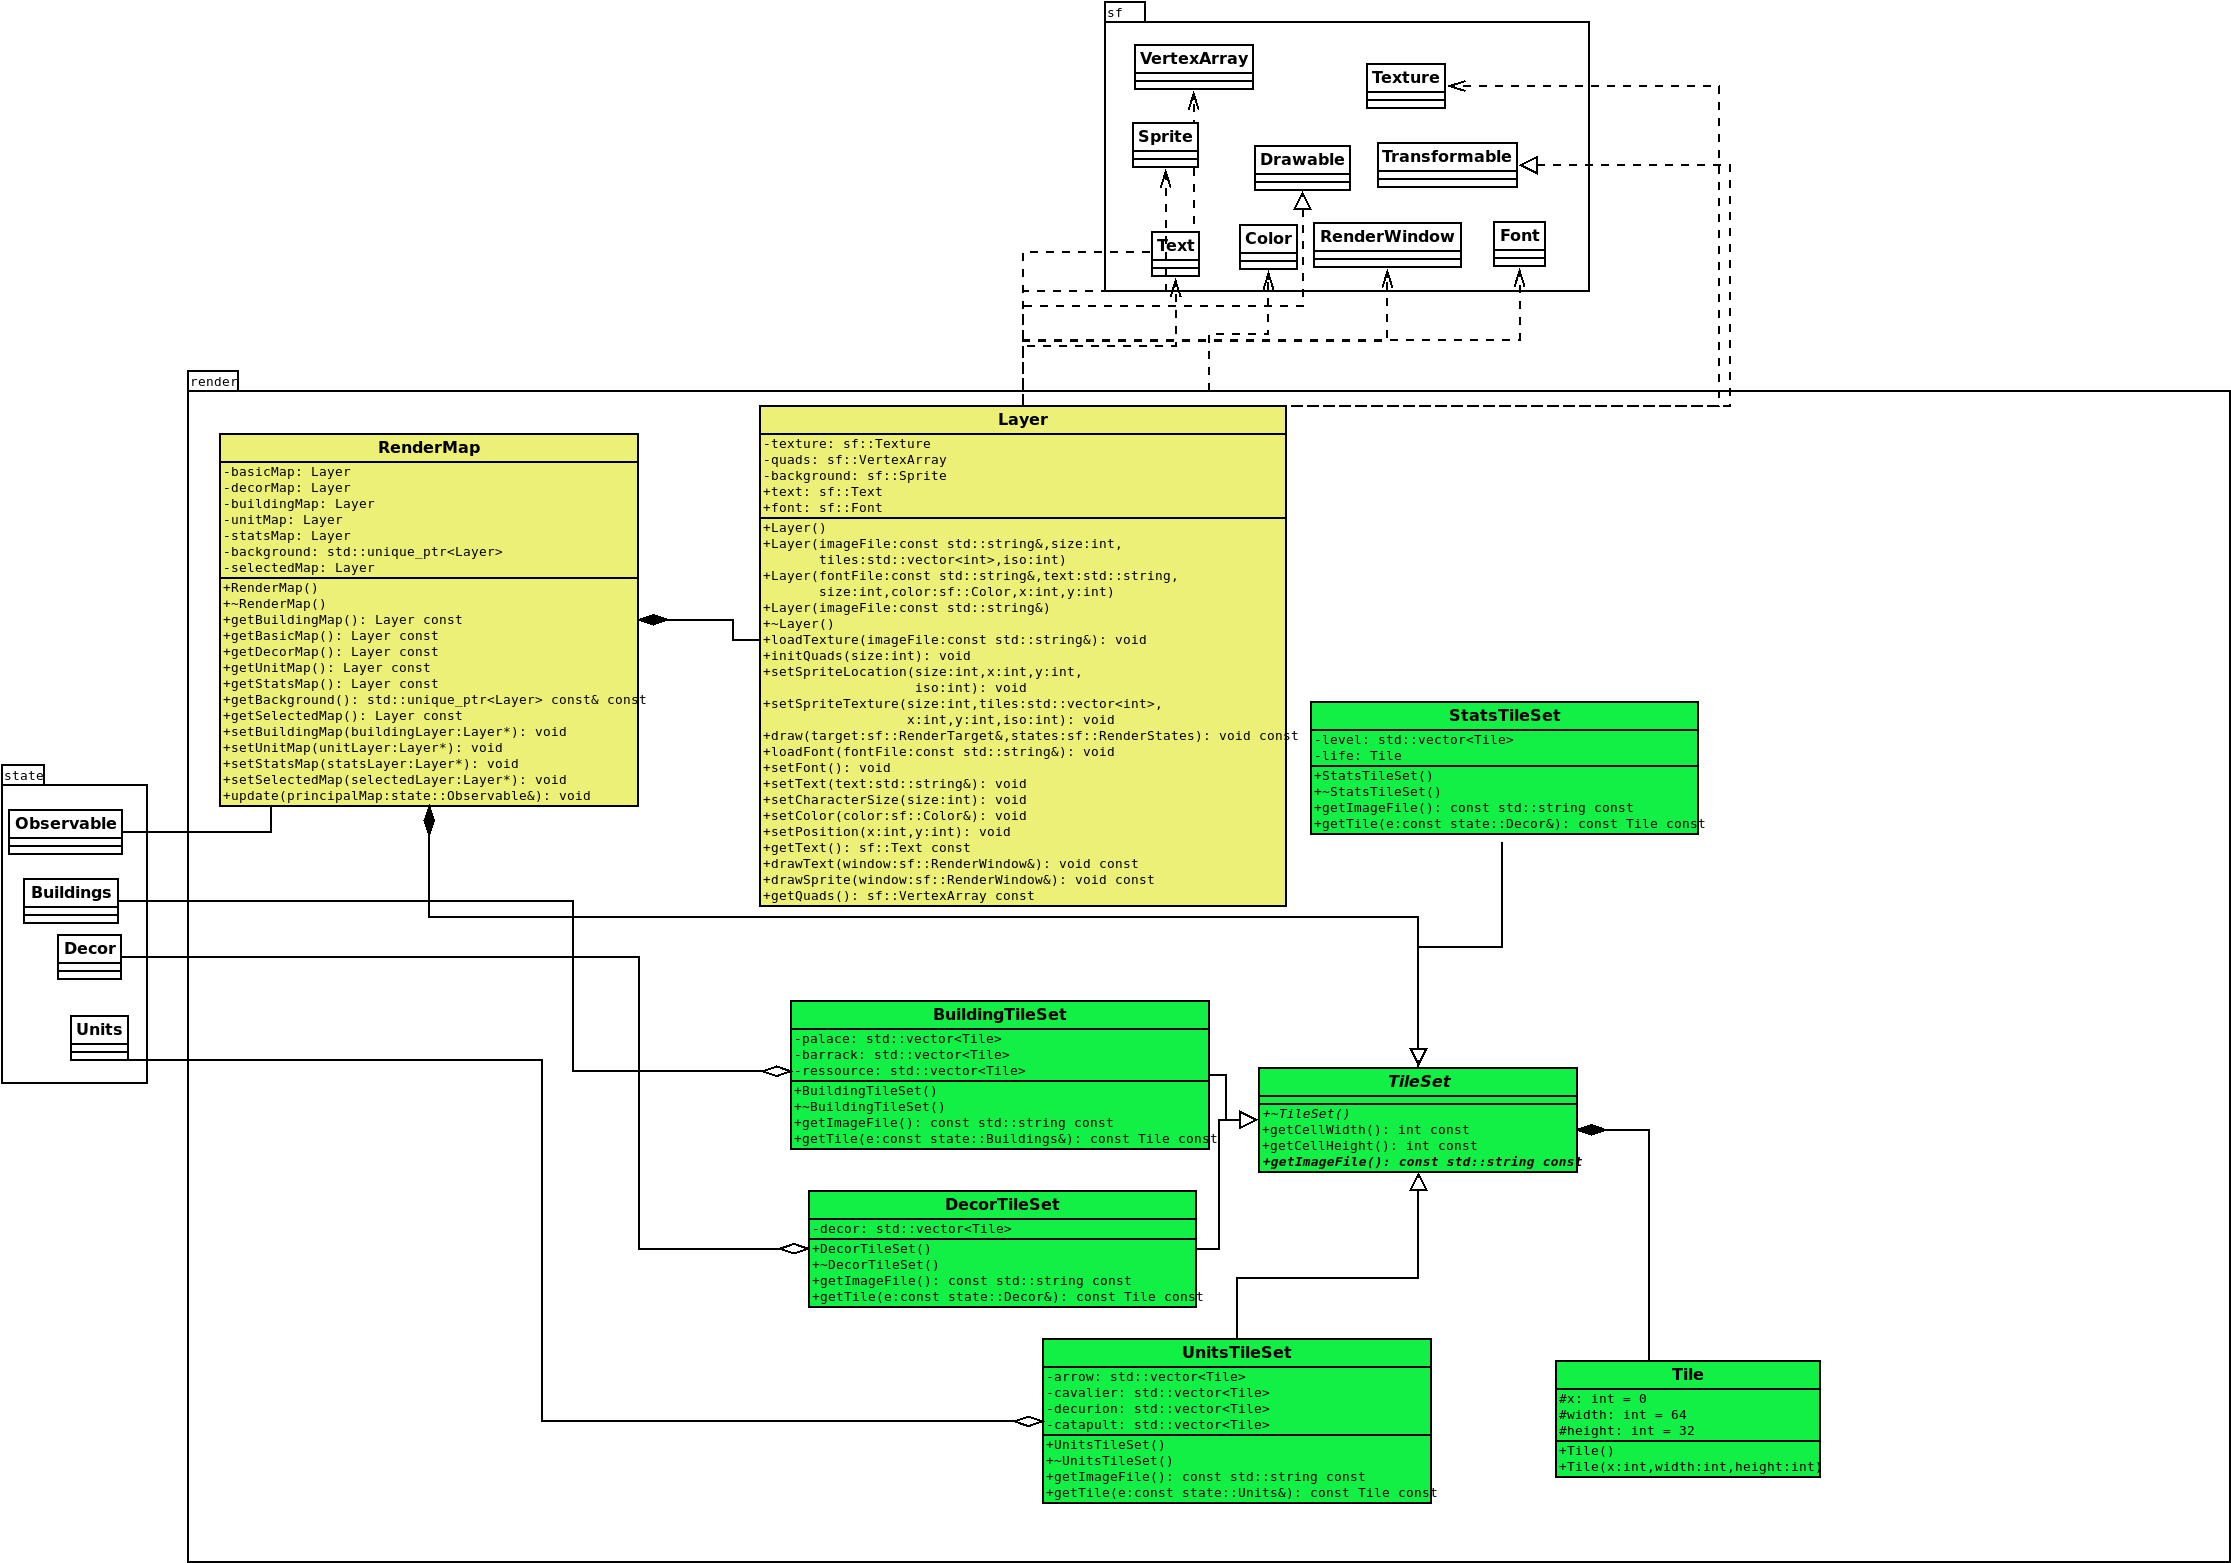
\includegraphics[width=1\textwidth]{ressources/render.png}
     \caption{Diagramme de classes du rendu}
\end{figure}

\newpage
\section{Règles de changements d'états et moteur de jeu}

\subsection{Horloge globale}
Tous les changements dans le jeu suivent une horloge globale pour le passage d'un état à un autre. \\
Ces changements sont réalisés en fonction du temps de passage d'un état à un autre. On attend la fin du changement d'état pour en réaliser un nouveau.

\subsection{Changements extérieurs}
Les changements extérieurs sont générés par des cliques du joueur. Les commandes sont les suivantes : 
\begin{itemize}
\item Cliquer sur n'importe quelle texture et consulter les actions qui lui sont associées ainsi que ses attributs (niveau de vie avec les coeurs, niveau, capacité ...).
\item Augmenter le niveau des bâtiments.
\item Créer des unités en séléctionnant leurs positions initiales avec un clique.
\item Déplacer des unités en choississant les cases parmi celles possibles.
\item Faire attaquer des unités entre elles.
\item Attaquer un hôtel de ville.
\end{itemize}

\subsection{Changements autonomes}
Ces changements sont ceux qui sont gérés par le moteur sans être provoqués par des actions utilisateurs
\begin{itemize}
\item Augmentation des ressources à chaque tour.
\item Disparition des unités qui n'ont plus de vie ainsi que de l'empire du palais n'ayant plus de vie.
\item Règles de mouvement et d'attaque.
\item Affichage des statistiques des bâtiments et des unités.
\end{itemize}


\subsection{Conception logiciel}
Le diagramme des classes du moteur est en figure 9 et diponible dans le dossier src du projet sous le nom de engine.
Dans cette étape de conception logiciel nous avons utilisé un pattern command. A son exécution, le moteur appelle des commandes en fonction des actions utilisateur.\\

\\Classes de commandes : Elles héritent toutes de la classe Command. Les commandes suivantes sont disponibles :
\begin{itemize}
\item CaseIdentifier : Permet d'identifier la case sur laquelle on se trouve.
\item Possibilities : Permet de déterminer quelles sont les actions possibles à partir de cette case.
\item PrintStats : Affiche les stats (vie, niveau, bouttons) des joueurs et des bâtiments.
\item LevelUp : Augmente le niveau d'un bâtiment.
\item CreateUnit : Créer une unité à partir d'un premier clique sur une caserne. Le second clique permet de positionner l'unité crée sur la map. Des boutons seront disponibles pour choisir le type d'unités à créer.
\item Move : Permet de déplacer une unité
\item Attack : Permet d'attaquer une unité ou un hôtel de ville.
\item Engine : implémente le moteur de jeu.
\end{itemize}

\begin{figure}[!ht]
\centering
    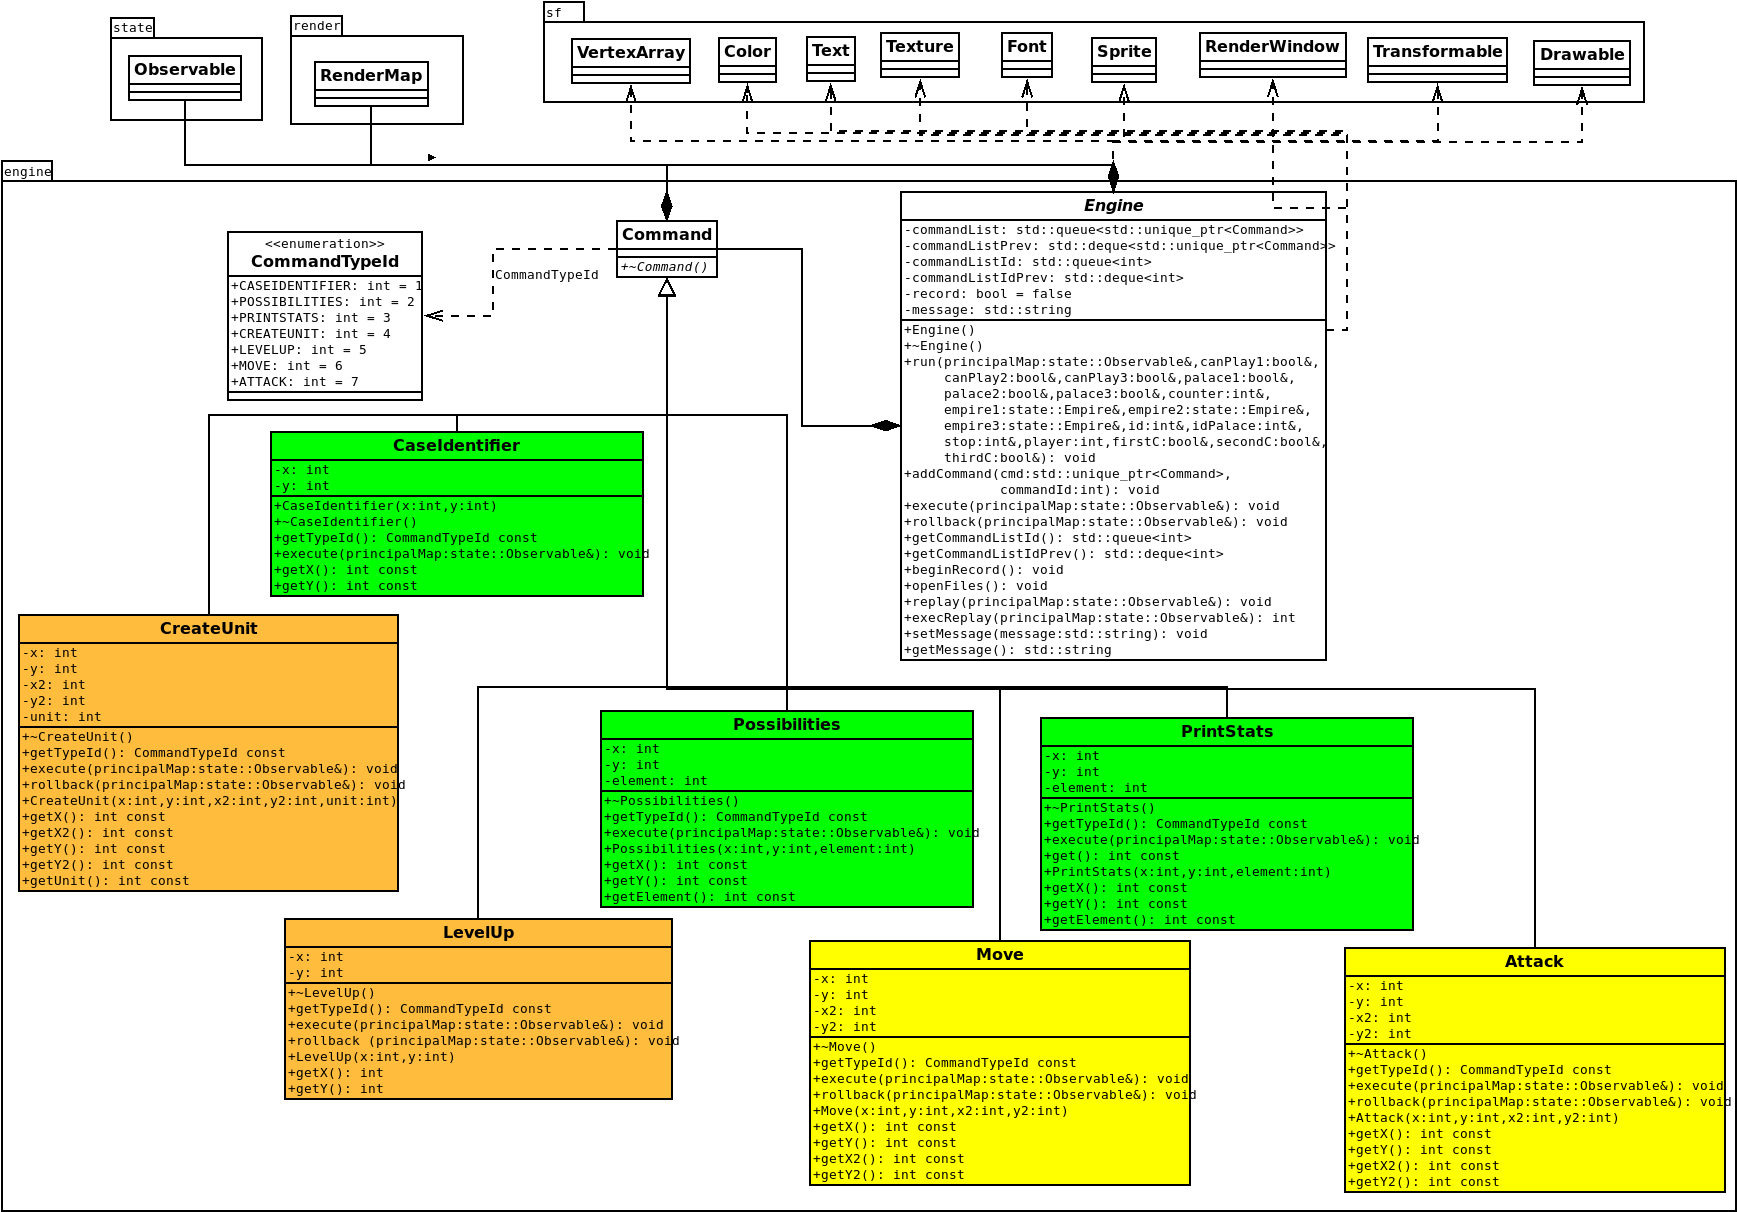
\includegraphics[width=1\textwidth]{ressources/engine.png}
     \caption{Diagramme de classes du moteur}
\end{figure}

\end{document}